\section{Evaluation}\label{sec:evaluation}

In this section, a quantitative evaluation of the proposed evolutionary tree cut algorithm is conducted.
The usefulness of our approach is then demonstrated with a case study.



\input{quantative_b.tex}

\subsection{Case Study}
This section highlights how \emph{RoseRiver} helps analyze large text streams by applying it to a news dataset, Obama data.
444,432 news articles that contain the keyword ``Obama,'' were collected from Sep. 1, 2012 to Jan. 14, 2013.
Grouped by week, the articles were organized into 18 topic trees. %(Fig.~\ref{fig:obamatree}).
%The average number of the first level nodes is 41, and the tree depth is 5($\pm 1$).
The tree depths varied from 4 to 5, the total node numbers changed from 144 to 297, and the node
number of the first level ranged from 18 to 79.
%\begin{figure}[ht]
%  \centering
%  \includegraphics[width=\columnwidth]{fig/obamatree}
%  \caption{Example topic tree for Obama data.}
%  \label{fig:obamatree}
%\end{figure}


To provide an overview of the news data to users, our system automatically extracted several initial focus nodes that can suitably represent the dataset and are distinct from one another.
In our implementation, a clustering method, the mean-shift algorithm, was utilized to cluster the topic at the first level because it is the most abstract level and can represent the topic tree very well.
Four clusters were detected in the Obama data.
For each cluster, we selected the node closest to the cluster center as a focus node.
Four focus nodes were automatically derived to generate the default overview (Fig.~\ref{fig:obama}(a)).
In the overview, the four colors represent four different topics: ``Iran'' (red), ``Tax'' (yellow), ``Debate'' (green), and ``Gun Control'' (purple).
As shown in Fig.~\ref{fig:obama}(a), significant variations existed; however, some overall patterns clearly stood out.
The green and yellow topics were dominant and divided the entire time period into two parts.
The red topic was small but persistent and the purple one was large but irruptive.

In the first half of the time period (before Nov. 3), the ``Debate'' (green) topic dominated and unsurprisingly ended in the week of Nov. 6, 2012, the date when Obama was reelected as president.
In addition, the ``Tax'' (yellow) topic was partially related to the ``Debate'' (green) topic from time to time.
Initially, the yellowish green topic (marked as \textbf{A} in Fig.~\ref{fig:obama}(a)), a mixed topic of ``Debate'' and ``Tax,'' merged with the green one.
This merging was caused by the tax-related debates (``Obama, Romney Clash on Economy, Taxes in First Debate'').
The yellowish green topic gradually split from the green one because its focus shifted to the economy, jobs, and the fiscal cliff.
If users are interested in tracking the mixed topic, they could interactively split the topic nodes and extract them from the green topic (Fig.~\ref{fig:obama}(b)).


Similarly, the ``Iran'' (red) topic  interacted with the ``Debate'' (green) topic in the week of Oct. 20 (marked as \textbf{B} in Fig.~\ref{fig:obama}(a)).
After splitting the topic nodes into small ones (Fig.~\ref{fig:obama}(c)), a red topic node that contained several news articles on ``Iran'' was observed
For example, one of the articles had the title ``Obama, Romney on Israel and Iran.'' This article clearly indicates why these two topics merged.

After the week of Nov. 3 (the second half of the time period), the ``Tax'' (yellow) topic dominated the view.
Considering that it has fewer connections with other topics, it was more isolated than the ``Debate'' topic.
Within these topics, the yellow nodes were almost fully connected with one another; thus, the ``Tax'' was also a relatively stable topic.

Although the ``Tax'' (yellow) topic was dominant during this time period, two greenish nodes (marked as \textbf{C} and \textbf{D} in Fig.~\ref{fig:obama}(a)) still appeared.
Clearly, these two topics have different evolution patterns.
Judging from the connections between \textbf{C} and the other nodes, \textbf{C} was likely a momentary topic.
To verify this hypothesis, we examined \textbf{C}'s content and found that it was focused on ``Romney blames loss on Obama's `gifts' to voters,'' which was indeed a momentary event.
On the other hand, \textbf{D} was fully connected to the yellow nodes. This connection indicates \textbf{D} contains news articles related to both the ``Debate'' and ``Tax'' topics. For example, one of the articles had the title ``GOP fights President Barack Obama on his campaign promise to raise taxes on the rich.''\looseness=-1


The ``Gun Control'' (purple) topic, which was caused by the Connecticut Elementary School massacre on Dec. 14, 2012, was then explored.
The event caused a topic burst in the week of Dec. 15.
Its horizontal offset indicates that it is a high-level topic node.
%Although the topic has a burst in the week of December 15, our system still finds several related topics, colored in purple, before the burst (marked as dotted rectangles in Fig.~\ref{fig:obama}(a)).
%Since they are highly related to our focus node, they are still successfully separated from the others.
%For example, in the week of Dec. 1, 2012 (marked as \textbf{E}), a node of only five documents talks about ``Obama to Push Gun Control in Second Term?''.
Then we split the big purple node and checked the two smaller topics in it (Fig.~\ref{fig:obama}(d)).
The lower node was mainly about the public discussion on gun control.
The strong connection of this node to the topic on the right indicates that it was still the major topic at the next time point.
When the node was split further, more detailed topics revealed themselves (Fig.~\ref{fig:obama}(e)).
From top to bottom, these topics were ``NRA calls for armed guards at every school,'' ``Obama turns to Biden on gun control measures,'' ``Guns fly off shelves,'' ``Assault weapons ban,'' and ``Connecticut school shooting: how to talk to your kids'' (marked as \textbf{F} to \textbf{J}, respectively).
The upper node, which represents follow-up news to the tragedy, has weaker connections to the right.
This condition indicates that the topic shrunk considerably at the next time point.

\begin{figure}[t]
  \vspace{-2mm}
  \centering
  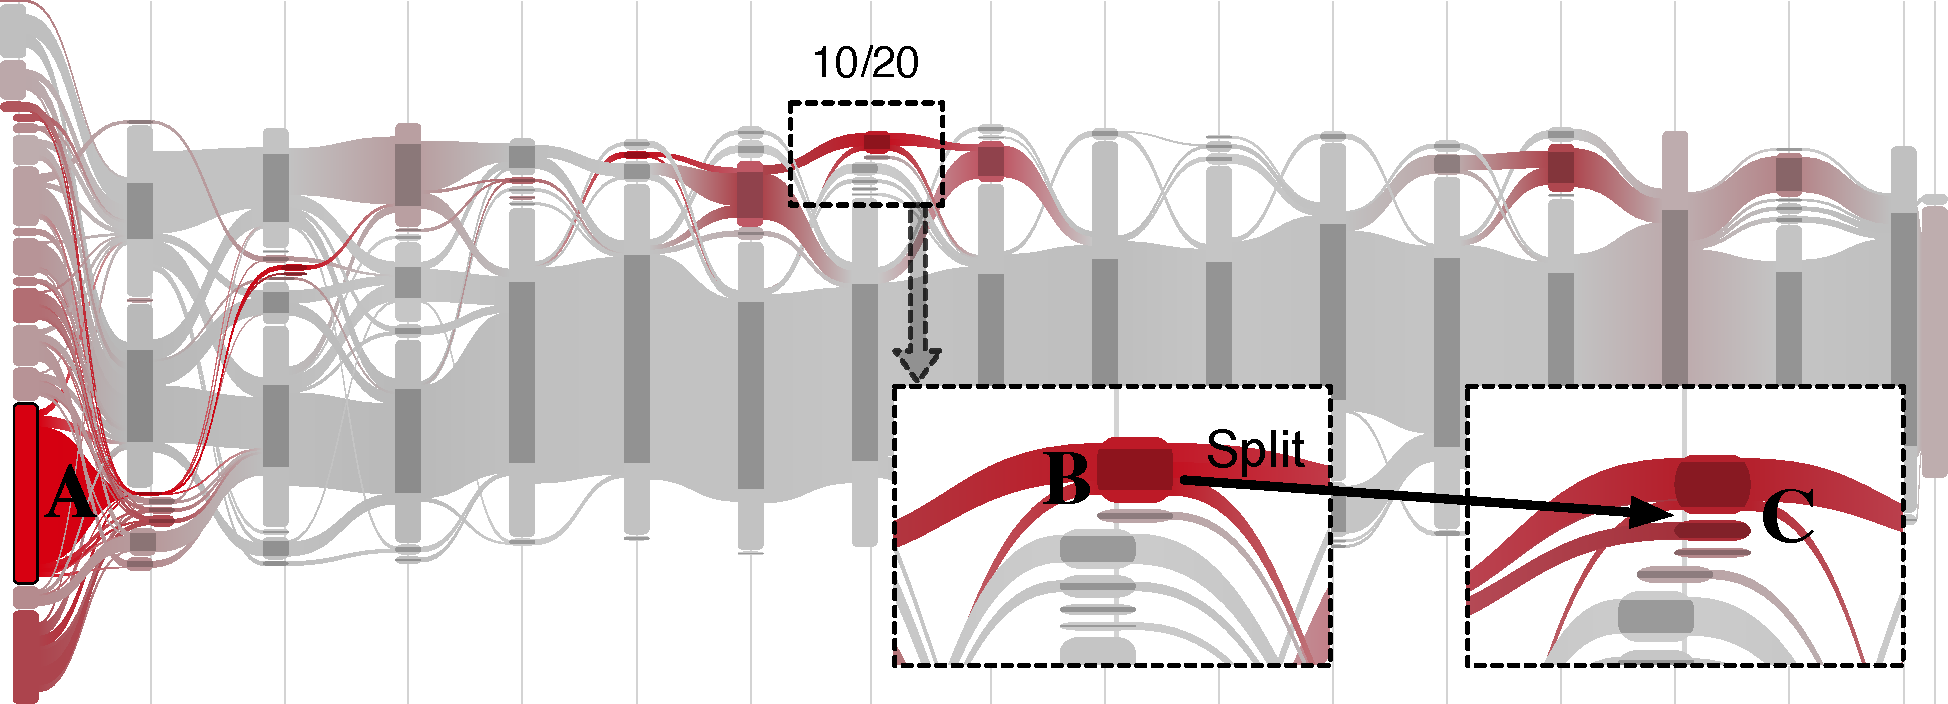
\includegraphics[width=\columnwidth]{fig/clintonoverview}
  \vspace{-5mm}
  \caption{``Bill Clinton'' related topics.}
  \label{fig:clintonoverview}

\end{figure}
%  \vspace{-4mm}

\begin{figure}[t]
  \centering
  \includegraphics[width=\columnwidth]{fig/2clintonoverview}
    \vspace{-3mm}
  \caption{Topics related to ``Bill Clinton'' and ``Hillary Clinton.''\looseness=-1}
  \vspace{-3mm}
  \label{fig:2clintonoverview}
\end{figure}

%from Shixia, the below story can be deleted if the qualitative evaluation need more space.



The search function can help users explore more specific topics.
For example, we entered ``Bill Clinton'' in the search box.
The first topic node recommended by our system is about the speech at the Democratic National Convention on Sep. 5, 2012.
We selected it as the focus node and visualized the result.
As shown in Fig.~\ref{fig:clintonoverview}, the topic was only active in the first week (marked as \textbf{A}).
However, in the week of Oct. 20, a small but highly related topic node appeared (marked as \textbf{B}).
We clicked it to see the detailed content and found that it contained two sub-topic nodes: ``Bill Clinton to rally for Obama at Springs Preserve'' and ``Hillary Clinton says she's `unlikely' to stay Secretary of State'' (marked as \textbf{C}).
To further explore these nodes, we regarded both nodes as new focus nodes and transformed the visualization.
Fig.~\ref{fig:2clintonoverview} shows that the two Clintons mainly have one overlapping topic (marked as \textbf{D}), which is ``Bill Clinton's DNC speech: Setting the stage for Hillary in 2016?''

%In the middle of Fig.~\ref{fig:2clintonoverview}, our tree cut algorithm successfully splits the context topic and reveals two small relevant topics hidden inside, which are a discussion about ``Poll: Clinton favored in 2016 in Iowa''.

The topics on Hillary Clinton in the top of Fig.~\ref{fig:2clintonoverview} can be  divided into two parts (marked by \textbf{F} and \textbf{G}).
\textbf{F} is about the Libya Attack, in which Hillary Clinton was highly involved.
In the week of Oct. 13, the article with the title ``Hillary Clinton Takes Blame for Benghazi Attack'' ended that topic (marked by \textbf{E}).
\textbf{G} contains two separate topics related to Hillary Clinton whose colors indicate that one is more relevant to the focus than the other.
In fact, the greener one is about Hillary Clinton herself.
For example, two articles have the titles ``Clinton is the people's choice for 2016 Prez bid: Poll,'' and ``Obama calls Clinton to wish her well as she recovers from concussion.''
However, the other is about the secretary of state candidates, in which Hillary Clinton is partially involved.



